\chapter{Introduction}

Anyone reading this book should be familiar with the notion of the first, second and higher derivatives, \textit{e.g.},for $f(t) = t^3 + 5 t^2 + 2$, 
\begin{align}
  \frac{df}{dt}(t) &= 3 t^2 + 10 t \\
  \frac{d^2f}{dt^2}(t) &= 6t + 10 \\
  \label{eq:derivs}
\end{align}
\textit{etc.} Also we naturally think of integrals in an antiderivative sense, \textit{e.g.},
\begin{align}
  \int f(t) dt &= \frac{1}{4} t^4 + \frac{5}{3} t^3 + 5 t^2 + c 
  \label{eq:integrals}
\end{align}
and we adopt a notation of $f^{(1)}(t)$ as the first derivative, $f^{(2)}(t)$ as the second derivative and $f^{(n)}(t)$ as the $n$th derivative as well as $f^{(-1)}(t)$ as $f$ integrated one time, $f^{(-2)}$ as $f$ integrated two times, \textit{etc.}

A mathematically curious reader may already be wondering if there are any derivatives ``between'' the integer ones. For example, is the a one-half derivative:
\begin{equation}
  \frac{d^\frac{1}{d} f}{d t^\frac{1}{2}}(t) = f^{\left(\frac{1}{2}\right)} = ?.
  \label{eq:halfderiv}
\end{equation}
There is not an immediate obvious answer to this because of the fact that the integer order derivative (as is the integral) is defined as a limit
\begin{equation}
  \frac{df}{dt}(t) = \lim_{\Delta t \rightarrow 0} = \frac{f\left(t + \Delta t \right) - f\left(t\right)}{\Delta t}
  \label{eq:limdef}
\end{equation}
and that is a discrete operation. There is not a natural half way to do it.

Basically we want to gereralize the notion of the derivative. In a sense, if we define something to give the, say $\alpha$ derivative where $\alpha \in \mathbb R$, \textit{i.e.}, $\alpha$ is a real number, then all we really need is that when $\alpha$ is an integer we get the usual definition of that integer order derivative. In between there may be lots of different options (there are!), but it makes sense to set some other basic requirements we want a fractional-order derivative to satisfy.

\begin{example}
  Consider $f(t) = t^2$ with the first and second derivatives $f^{(1)}(t) = 2 t$ and $f^{(2)}(t) = 2$, respectively. We should expect that the $1/2$ derivative is, in some qualitative sense, ``between'' $f(t)$ and $f^{(1)}(t)$, and that the $3/2$ derivative is ``between'' the first and second derivatives. 

  % GNUPLOT: LaTeX picture with Postscript
\begingroup
  \makeatletter
  \providecommand\color[2][]{%
    \GenericError{(gnuplot) \space\space\space\@spaces}{%
      Package color not loaded in conjunction with
      terminal option `colourtext'%
    }{See the gnuplot documentation for explanation.%
    }{Either use 'blacktext' in gnuplot or load the package
      color.sty in LaTeX.}%
    \renewcommand\color[2][]{}%
  }%
  \providecommand\includegraphics[2][]{%
    \GenericError{(gnuplot) \space\space\space\@spaces}{%
      Package graphicx or graphics not loaded%
    }{See the gnuplot documentation for explanation.%
    }{The gnuplot epslatex terminal needs graphicx.sty or graphics.sty.}%
    \renewcommand\includegraphics[2][]{}%
  }%
  \providecommand\rotatebox[2]{#2}%
  \@ifundefined{ifGPcolor}{%
    \newif\ifGPcolor
    \GPcolorfalse
  }{}%
  \@ifundefined{ifGPblacktext}{%
    \newif\ifGPblacktext
    \GPblacktexttrue
  }{}%
  % define a \g@addto@macro without @ in the name:
  \let\gplgaddtomacro\g@addto@macro
  % define empty templates for all commands taking text:
  \gdef\gplbacktext{}%
  \gdef\gplfronttext{}%
  \makeatother
  \ifGPblacktext
    % no textcolor at all
    \def\colorrgb#1{}%
    \def\colorgray#1{}%
  \else
    % gray or color?
    \ifGPcolor
      \def\colorrgb#1{\color[rgb]{#1}}%
      \def\colorgray#1{\color[gray]{#1}}%
      \expandafter\def\csname LTw\endcsname{\color{white}}%
      \expandafter\def\csname LTb\endcsname{\color{black}}%
      \expandafter\def\csname LTa\endcsname{\color{black}}%
      \expandafter\def\csname LT0\endcsname{\color[rgb]{1,0,0}}%
      \expandafter\def\csname LT1\endcsname{\color[rgb]{0,1,0}}%
      \expandafter\def\csname LT2\endcsname{\color[rgb]{0,0,1}}%
      \expandafter\def\csname LT3\endcsname{\color[rgb]{1,0,1}}%
      \expandafter\def\csname LT4\endcsname{\color[rgb]{0,1,1}}%
      \expandafter\def\csname LT5\endcsname{\color[rgb]{1,1,0}}%
      \expandafter\def\csname LT6\endcsname{\color[rgb]{0,0,0}}%
      \expandafter\def\csname LT7\endcsname{\color[rgb]{1,0.3,0}}%
      \expandafter\def\csname LT8\endcsname{\color[rgb]{0.5,0.5,0.5}}%
    \else
      % gray
      \def\colorrgb#1{\color{black}}%
      \def\colorgray#1{\color[gray]{#1}}%
      \expandafter\def\csname LTw\endcsname{\color{white}}%
      \expandafter\def\csname LTb\endcsname{\color{black}}%
      \expandafter\def\csname LTa\endcsname{\color{black}}%
      \expandafter\def\csname LT0\endcsname{\color{black}}%
      \expandafter\def\csname LT1\endcsname{\color{black}}%
      \expandafter\def\csname LT2\endcsname{\color{black}}%
      \expandafter\def\csname LT3\endcsname{\color{black}}%
      \expandafter\def\csname LT4\endcsname{\color{black}}%
      \expandafter\def\csname LT5\endcsname{\color{black}}%
      \expandafter\def\csname LT6\endcsname{\color{black}}%
      \expandafter\def\csname LT7\endcsname{\color{black}}%
      \expandafter\def\csname LT8\endcsname{\color{black}}%
    \fi
  \fi
    \setlength{\unitlength}{0.0500bp}%
    \ifx\gptboxheight\undefined%
      \newlength{\gptboxheight}%
      \newlength{\gptboxwidth}%
      \newsavebox{\gptboxtext}%
    \fi%
    \setlength{\fboxrule}{0.5pt}%
    \setlength{\fboxsep}{1pt}%
\begin{picture}(5832.00,3600.00)%
\definecolor{gpBackground}{rgb}{1.000, 1.000, 1.000}%
\put(0,0){\colorbox{gpBackground}{\makebox(5832.00,3600.00)[]{}}}%
    \gplgaddtomacro\gplbacktext{%
      \colorrgb{0.15,0.15,0.15}%%
      \put(740,640){\makebox(0,0)[r]{\strut{}-10}}%
      \colorrgb{0.15,0.15,0.15}%%
      \put(740,1330){\makebox(0,0)[r]{\strut{}-5}}%
      \colorrgb{0.15,0.15,0.15}%%
      \put(740,2020){\makebox(0,0)[r]{\strut{}0}}%
      \colorrgb{0.15,0.15,0.15}%%
      \put(740,2709){\makebox(0,0)[r]{\strut{}5}}%
      \colorrgb{0.15,0.15,0.15}%%
      \put(740,3399){\makebox(0,0)[r]{\strut{}10}}%
      \colorrgb{0.15,0.15,0.15}%%
      \put(860,440){\makebox(0,0){\strut{}-3}}%
      \colorrgb{0.15,0.15,0.15}%%
      \put(1629,440){\makebox(0,0){\strut{}-2}}%
      \colorrgb{0.15,0.15,0.15}%%
      \put(2397,440){\makebox(0,0){\strut{}-1}}%
      \colorrgb{0.15,0.15,0.15}%%
      \put(3166,440){\makebox(0,0){\strut{}0}}%
      \colorrgb{0.15,0.15,0.15}%%
      \put(3934,440){\makebox(0,0){\strut{}1}}%
      \colorrgb{0.15,0.15,0.15}%%
      \put(4703,440){\makebox(0,0){\strut{}2}}%
      \colorrgb{0.15,0.15,0.15}%%
      \put(5471,440){\makebox(0,0){\strut{}3}}%
    }%
    \gplgaddtomacro\gplfronttext{%
      \colorrgb{0.15,0.15,0.15}%%
      \put(190,2019){\rotatebox{90}{\makebox(0,0){\strut{}function and derivatives}}}%
      \colorrgb{0.15,0.15,0.15}%%
      \put(3165,140){\makebox(0,0){\strut{}$t$}}%
    }%
    \gplbacktext
    \put(0,0){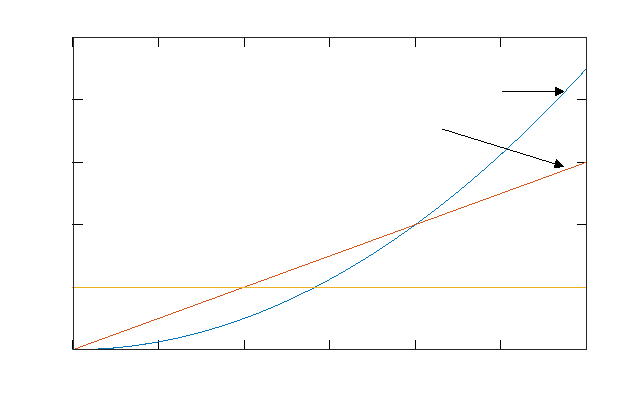
\includegraphics[width={291.60bp},height={180.00bp}]{fracidea}}%
    \gplfronttext
  \end{picture}%
\endgroup

\end{example}

